\documentclass[11pt]{article}
\usepackage{scribe}
\usepackage{graphicx}

% Uncomment the appropriate line
%\Scribe{Your name}

\Scribes{Frendy Lio Can}
\LectureDate{October 5, 2020}
\LectureTitle{Homework Assignment \#2}

%\usepackage[mathcal]{euscript}


\begin{document}

\MakeScribeTop

%\paragraph{This is a paragraph heading} Paragraph.

%%%%%%%%%%%%%%%%%%%%%%%%%%%%%%%%
% PROBLEM 1
%%%%%%%%%%%%%%%%%%%%%%%%%%%%%%%%
\paragraph{\noindent\textbf{\LARGE{Problem 1, a)}}}

% Start of Explaining

\begin{flushleft}
Is this linear system? 
\newline
\newline
Let:
\end{flushleft}   
\begin{equation*}
\begin{split}
    g[m,n]      = & \sum_{k-1}^1 \sum_{l-1}^1 x[m-k, n-l] \\
    y_1[m,n]    = & x_1[m, n] + \lambda (x_1[m,n] - \frac{1}{9}g_1[m,n]) \\
    y_2[m,n]    = & x_2[m, n] + \lambda (x_2[m,n] - \frac{1}{9}g_2[m,n])
\end{split}
\end{equation*}
    


\begin{flushleft}
Lets check if scaling property holds:
\end{flushleft}   
\begin{equation*}
\begin{split}
    x_s[m.n]    =& \alpha x_1[m,n] \\
    g_s[m,n]    =& \alpha g_1[m,n] \\
    y_s[m.n]    =& \alpha y_1[m,n] \\
    y_s[m,n]    =& x_s[m, n] + \lambda (x_s[m,n] - \frac{1}{9}g_s[m,n]) \\
                =& \alpha x_1[m,n] + \lambda (\alpha x_1[m,n] - \frac{1}{9}\alpha g_1[m,n]) \\
                =& \alpha [x_1[m, n] + \lambda (x_1[m,n] - \frac{1}{9}g_1[m,n])] \\
                =& \alpha y_1[m,n]
\end{split}
\end{equation*}

\begin{flushleft}
    Thus, the scaling property is true.
\end{flushleft} 

\begin{flushleft}
Lets check if additive property holds:
\end{flushleft}   
\begin{equation*}
\begin{split}
    x_s[m.n]    =& x_1[m,n] + x_2[m,n] \\
    g_s[m,n]    =& g_1[m,n] + g_2[m,n] \\
    y_s[m.n]    =& y_1[m,n] + y_2[m,n] \\
    y_s[m,n]    =& x_s[m, n] + \lambda (x_s[m,n] - \frac{1}{9}g_s[m,n]) \\
                =& x_1[m,n] + x_2[m,n] + \lambda (x_1[m,n] + x_2[m,n] - \frac{1}{9}(g_1[m,n] + g_2[m,n])) \\
                =& x_1[m, n] + \lambda (x_1[m,n] - \frac{1}{9}g_1[m,n]) +  x_2[m, n] + \lambda (x_2[m,n] - \frac{1}{9}g_2[m,n]) \\
                =& y_1[m,n] + y_2[m,n]
\end{split}
\end{equation*}

\begin{flushleft}
    Thus, the additive property is true. 
    \newline
    \newline
    Since the scale and additive property are true, this implies that $y[m,n]$ is a linear system.
    \newline
    \newline
    Is this a space invariant system?
\end{flushleft} 
\begin{equation*}
\begin{split}
    x_s[m.n]    =& x_1[m - m_0,n - n_0]\\
    g_s[m,n]    =& g_1[m - m_0,n - n_0] \\
    y_s[m.n]    =& y_1[m - m_0,n - n_0] \\
    y_s[m,n]    =& x_s[m, n] + \lambda (x_s[m,n] - \frac{1}{9}g_s[m,n]) \\
                =& x_1[m - m_0,n - n_0] + \lambda (x_1[m - m_0,n - n_0] - \frac{1}{9}g_1[m - m_0,n - n_0]) \\
                =& y_1[m - m_0,n - n_0]
\end{split}
\end{equation*}
\begin{flushleft}
    Thus, it is  space invariant.
    \newline
    \newline
    To conclude, $y[m,n]$ is a linear system and space invariant.
\end{flushleft} 

% ==================
% ==================
\paragraph{\noindent\textbf{\LARGE{Problem 1, b)}}}  
\begin{flushleft}
    If 2D impulse response:
\end{flushleft} 
\begin{equation*}
\begin{split}
    x[m,n]  = & \delta[m,n] \\
    g[m,n]  = & \sum_{k-1}^1 \sum_{l-1}^1 \delta[m-k, n-l] 
\end{split}
\end{equation*}
\begin{flushleft}
    Thus:
\end{flushleft} 
\begin{equation*}
\begin{split}
    h[m,n] = & \delta[m,n] + \lambda (\delta[m,n] - \frac{1}{9}g[m,n])
\end{split}
\end{equation*}

\begin{flushleft}
    We also know that $\delta[m,n] = 1$ , when $m \wedge n = 0$. Therefore:
\end{flushleft} 
\begin{equation*}
    h[m,n] =
    \begin{cases}
      1 + \frac{8}{9}\lambda & \text{if } m \wedge n = 0 \\
      -\lambda \frac{1}{9} & \text{if }  -1 \leq m \wedge n \leq 1 \text{,but no } m \wedge n = 0\\
      0 & \text{otherwise}
    \end{cases} 
\end{equation*}

% ==================
% ==================
\paragraph{\noindent\textbf{\LARGE{Problem 1, c)}}}  
\begin{equation*}
\begin{split}
    g[m,n]  = & \sum_{k-1}^1 \sum_{l-1}^1 \delta[m-k, n-l]  \\
    H(e^{i\mu}, e^{i\nu}) = &\sum_{m,n = -\infty }^\infty h[m,n] e^{-i(\mu m + \nu n)} \\
                        = & \sum_{m,n = -\infty }^\infty \delta[m,n] + \lambda (\delta[m,n] - \frac{1}{9}g[m,n]) e^{-i(\mu m + \nu n)} \\
                        = & (1 + \lambda)(e^{-i(\mu 0 + \nu 0)} )  - \lambda \frac{1}{9} [\\
                        & \quad [(e^{-i(\mu (-1) + \nu (-1))}) + (e^{-i(\mu (-1) + \nu (0))}) + ( e^{-i(\mu (-1) + \nu (1))})] +\\
                        & \quad [(e^{-i(\mu (0) + \nu (-1))}) + (e^{-i(\mu (0) + \nu (0))}) + ( e^{-i(\mu (0) + \nu (1))})] +\\
                        & \quad [(e^{-i(\mu (1) + \nu (-1))}) + (e^{-i(\mu (1) + \nu (0))}) + ( e^{-i(\mu (1) + \nu (1))})] ]\\
                        = & 1 + \lambda - \lambda \frac{1}{9} [ \\
                        & \quad [(e^{i(\mu + \nu)})+(e^{i\mu})+(e^{i(\mu - \nu)})] + \\
                        & \quad [(e^{i(\nu)})+(e^{0})+(e^{i(-\nu)})] + \\
                        & \quad [(e^{-i(\mu - \nu)})+(e^{-i\mu})+(e^{-i(\mu + \nu)})]  \\
                        = & 1 + \lambda - \lambda \frac{1}{9} [ \\
                        & \quad [e^{i\mu}((e^{i\nu})+ (1) + (e^{- i\nu}))] + \\
                        & \quad [(e^{i\nu})+ (1) + (e^{- i\nu})] + \\
                        & \quad  [e^{-i\mu}((e^{i\nu})+ (1) + (e^{- i\nu}))]  \\
                        = & 1 + \lambda - \lambda \frac{1}{9} ((e^{i\mu})+ (1) + (e^{- i\mu}))((e^{i\mu})+ (1) + (e^{- i\nu})) \\
                        = & 1 + \lambda - \lambda \frac{1}{9} ( 2cos(\mu) + 1)(2 cos(\nu) + 1)
\end{split}
\end{equation*}

%%%%%%%%%%%%%%%%%%%%%%%%%%%%%%%%
% PROBLEM 2
%%%%%%%%%%%%%%%%%%%%%%%%%%%%%%%%
\paragraph{\noindent\textbf{\LARGE{Problem 1, d)}}}
\begin{flushleft}
    High-Pass Filter
    \\
    We can observe that the the filter will be approximately $\lambda \frac{8}{9} ( 2cos(\mu) + 1)(2 cos(\nu) + 1)$.
\\
 This clearly shows that is a high pass filter as this filter will sharpen an image. 

\end{flushleft} 

%%%%%%%%%%%%%%%%%%%%%%%%%%%%%%%%
% PROBLEM 2
%%%%%%%%%%%%%%%%%%%%%%%%%%%%%%%%
\paragraph{\noindent\textbf{\LARGE{Problem 1, e)}}}    
\begin{flushleft}
    Low-Pass Filter.
    \\
    We can observe that the the filter will be approximately $\frac{1}{9} ( 2cos(\mu) + 1)(2 cos(\nu) + 1)$.
\\
 This clearly shows that is a low pass filter as this filter will blur an image. 
\end{flushleft} 


%%%%%%%%%%%%%%%%%%%%%%%%%%%%%%%%
% PROBLEM 2
%%%%%%%%%%%%%%%%%%%%%%%%%%%%%%%%
\newpage
\paragraph{\noindent\textbf{\LARGE{Problem 2, a)}}}    
\begin{equation*}
\begin{split}
    H(e^{i\mu}, e^{i\nu}) = &\sum_{m,n = -\infty }^\infty h[m,n] e^{-i(\mu m + \nu n)} \\
                        = & \sum_{m,n = -2 }^2 \frac{1}{25} e^{-i(\mu m + \nu n)} + 0\\
                        = & \frac{1}{25} (e^{i2\mu} + e^{i\mu} + e^0 + e^{-i\mu} + e^{-i2\mu}) (e^{i2\nu} + e^{i\nu} + e^0 + e^{-i\nu} + e^{-i2\nu}) \\
                        = & \frac{1}{25} (2 cos(2 \mu) + 2 cos(\mu) + 1) (2 cos(2 \nu) + 2 cos(\nu) + 1)
\end{split}
\end{equation*}

\begin{figure}[htbp]
    \centerline{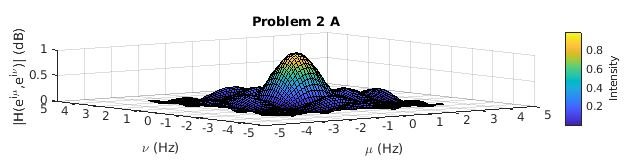
\includegraphics[scale=.5]{2A.JPG}}
    \caption{Problem 2-a)}
    \label{fig}
\end{figure}

\paragraph{\noindent\textbf{\LARGE{Problem 2, b)}}}    
\begin{equation*}
\begin{split}
    G(e^{i\mu}, e^{i\nu}) = &\sum_{m,n = -\infty }^\infty g[m,n] e^{-i(\mu m + \nu n)} \\
    = & \sum_{m,n = -\infty }^\infty (\delta[m,n] + \lambda \delta[m,n] - \lambda h[m,n]) e^{-i(\mu m + \nu n)} \\                    
    = & 1 + \lambda - \lambda H(e^{i\mu}, e^{i\nu}) \\
    H(e^{i\mu}, e^{i\nu}) = &  \frac{1}{25} (2 cos(2 \mu) + 2 cos(\mu) + 1) (2 cos(2 \nu) + 2 cos(\nu) + 1)
\end{split}
\end{equation*}

\begin{figure}[htbp]
    \centerline{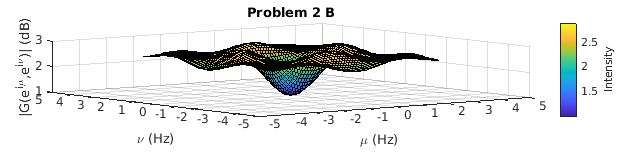
\includegraphics[scale=.5]{2B.JPG}}
    \caption{Problem 2-b)}
    \label{fig}
\end{figure}

\end{document}
